\documentclass[reqno, 12pt]{amsart}
\usepackage{style}

\title[Lecture Notes]{Math 142: Lecture Notes}
\author{Blake Farman}
\date{February 6, 2018}

\begin{document}
\maketitle

\section{Numerical Integration}
The idea of this section is to be able to estimate integrals of functions for which there are no known elementary antiderivatives with methods which are generally \lq better\rq\ than simply using rectangles.
Both of the methods in this section have the advantage of being extremely straightforward to implement in your favorite mathematics software (Sage, Mathematica, Matlab, Maple, etc.).

For ease of presentation, we make some simplifications.
We will assume throughout that \(f\) is a non-negative, continuous function on \([a,b]\), however it need only be continuous in \([a,b]\) for this to work.
\subsection{Trapezoidal Approximations}

Let \(\Delta x = \frac{b - a}{n}\) and take the partition
\[x_0 = a,\, x_1 = a + \Delta x,\, x_2 = a + 2\Delta x,\, \ldots,\, x_{n-1} = a + (n-1)\Delta x,\, x_n = b.\]
We name the function values
\[y_0 = f(a),\, y_1 = f(x_1),\, \ldots,\, y_n = f(x_n)\]
and, on each subinterval \([x_i, x_{i + 1}]\), we construct a trapezoid connecting the points \([x_i,y_i]\) and \([x_{i+1}, y_{i+1}]\) to get something that looks like the following
\begin{center}
  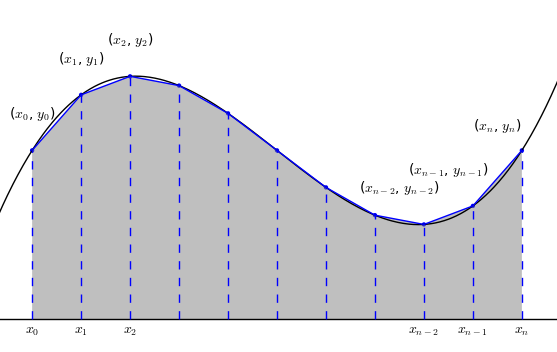
\includegraphics[scale=0.5]{trapezoid}
\end{center}

To estimate the integral
\[\int_a^b f(x)\dif x\]
we need only sum the areas of the trapezoids.
The \(i^\text{th}\) trapezoid looks like
\begin{center}
  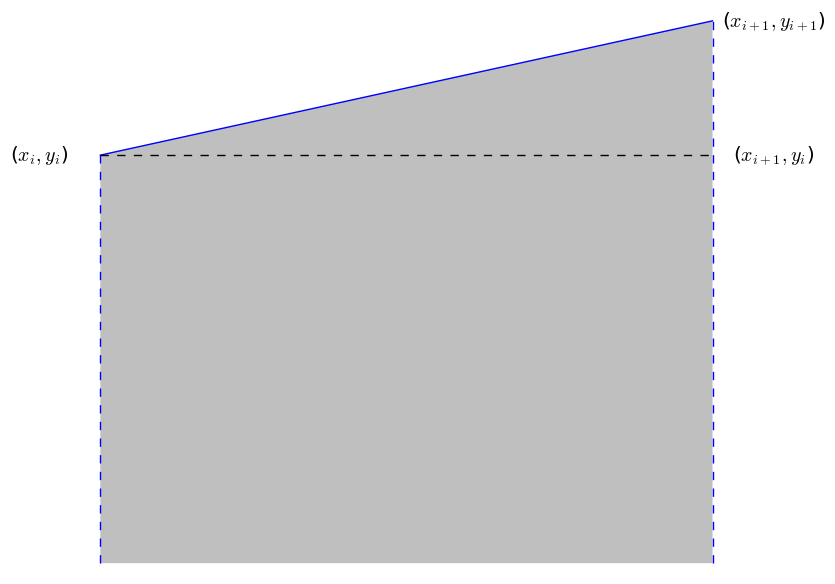
\includegraphics[scale=0.5]{singleTrap}
\end{center}
so its area can be computed as the sum of the area of the triangle on top and the area of the rectangle on the bottom
\[\frac{1}{2}(y_{i+1} - y_i)\Delta x + y_i \Delta x = \frac{1}{2}(y_{i+1} - y_i + 2y_i)\Delta x = \frac{y_{i} + y_{i+1}}{2}\Delta x.\]
To get an approximation to the area underneath the curve \(f\) we now add up the areas of the \(n\) trapezoids
\begin{gather*}
  \frac{y_0 + y_1}{2}\Delta x + \frac{y_1 + y_2}{2}\Delta x + \ldots + \frac{y_{n-2} + y_{n - 1}}{2}\Delta x + \frac{y_{n-1} + y_n}{2}\Delta x \\
  = (y_0 + y_1 + y_1 + y_2 + \ldots y_{n-2} + y_{n-1} + y_{n-1} + y_n)\frac{\Delta x}{2}.
\end{gather*}
We observe that \(y_0\) and \(y_n\) appear in the sum only once, but each other \(y_i\) appears twice: once on the subinterval \([x_i, x_{i+1}]\) and once on the subinterval \([x_{i+1}, x_{i+2}]\).
Therefore we have
\begin{theorem}[The Trapezoidal Rule]
  To approximate the integral
  \[\int_a^b f(x)\dif x\]
  by \(n\) trapezoids of base width
  \[\Delta x = \frac{b - a}{2}\]
  use
  \[T = (y_0 + 2y_1 + 2y_2 + \ldots + 2y_{n-2} + 2y_{n-1} + y_n)\frac{\Delta x}{2} \]
  where
  \[x_0 = a,\, x_1 = a + \Delta x,\, x_2 = a + 2\Delta x,\, \ldots,\, x_{n-1} = a + (n-1)\Delta x,\, x_n = b\]
  and \(y_i = f(x_i)\) for \(0 \leq i \leq n\).
\end{theorem}

\begin{example}
  Use the Trapezoidal Rule to approximate
  \[\int_1^2 x^2 \dif x\]
  using \(n = 4\) trapezoids.
\end{example}
\begin{proof}[Solution]
  First we compute
  \[\Delta x = \frac{2 - 1}{4} = \frac{1}{4}\]
  so our partition is
  \[x_0 = 1,\, x_1 = 5/4,\, x_2 = 3/2,\, x_3 = 7/4,\, x_4 = 2\]
  and
  \[y_0 = 1,\, y_1 = \frac{25}{16},\, y_2 = \frac{9}{4},\, y_3 = \frac{49}{16},\, y_4 = 4.\]
  We can sketch the trapezoids we're using for our approximation
  \begin{center}
    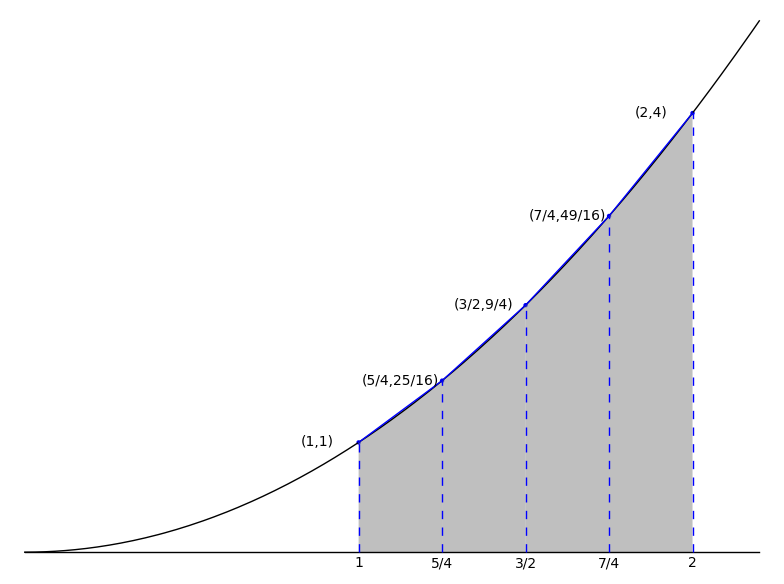
\includegraphics[scale=0.5]{trapParabola}
  \end{center}
  The estimate is then
  \begin{eqnarray*}
    T &=& \left(1 + 2\cdot\frac{25}{16} + 2\cdot\frac{9}{4} + 2\cdot\frac{49}{16} + 4\right)\frac{1/4}{2}\\
    &=& \left(\frac{8}{8} + \frac{25}{8} + \frac{36}{8} + \frac{49}{8} + \frac{32}{8}\right)\frac{1}{8}\\
    &=& \frac{150}{64}\\
    &=& \frac{75}{32}
  \end{eqnarray*}

  Since we know how to compute the actual area, we see that the estimate has an error of
  \begin{eqnarray*}
    \int_1^2 x^2 \dif x - \frac{75}{32} &=& \frac{2^3 - 1^3}{3} - \frac{75}{32}\\
    &=& \frac{7}{3} - \frac{75}{32}\\
    &=& \frac{7(32) - 3(75)}{96}\\
    &=& \frac{210 + 14 - 210 - 15}{96}\\
    &=& -\frac{1}{96}\\
    &=& -0.01041\overline{6}.
  \end{eqnarray*}
  Thus the trapezoidal rule gives a slight over-estimate here.
\end{proof}

\subsection{Simpson's Rule: Approximations Using Parabolas}

Once again, we let
\[\Delta x = \frac{b - a}{2},\]
take an evenly spaced partition
\[x_0 = a,\, x_1 = a + \Delta x,\, x_2 = a + 2\Delta x,\, \ldots,\, x_{n-1} = a + (n-1)\Delta x,\, x_n = b,\]
and denote \(y_i = f(x_i)\) for \(0 \leq i \leq n\).
However, this time we require that \textbf{\(n\) is an even integer}.

We make this stipulation because we will fit a parabola to three points
\[(x_{i-1}, y_{i-1}), (x_i, y_i), (x_{i+1},y_{i+1})\]
and use the area under the parabola on the interval \([x_{i-1}, x_{i+1}]\) as an estimate for
\[\int_{x_i-1}^{x_{i+1}} f(x)\dif x = \int_{x_{i-1}}^{x_i} f(x)\dif x + \int_{x_i}^{x_{i+1}}f(x)\dif x.\]
Since the partition subdivides \([a,b]\) into \(n\) subintervals and each parabola estimates the area on two of these subintervals, we must use \(n/2\) parabolas, and hence \(n\) \textbf{must} be even for the method to work.

To get a feel for what is happening here, depicted below is a curve with a parabola fitted to the three points
\[(x_2,y_2), (x_3,y_3), (x_4,y_4).\]
The shaded region represents the area under the parabola, \(p(x)\), which approximates the area under the curve \(f\) on the interval \([x_2,x_4]\).
\begin{center}
  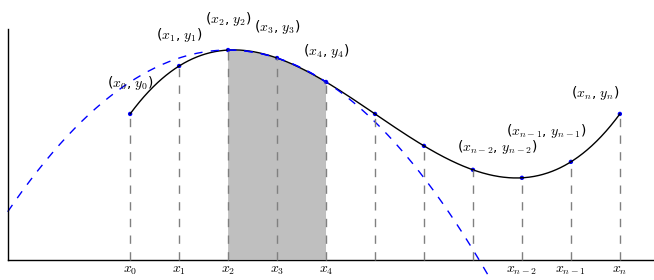
\includegraphics[scale=0.5]{simpson}
\end{center}
For each of the \(m = n/2\) subintervals,
\[[x_1, x_3], [x_2,x_4], \ldots, [x_{n-4}, x_{n-2}], [x_{n-2}, x_n]\]
we must compute the area under the parabolas and then sum them up.
To make our task a little simpler, we make the following observation.

We note that if we shift our graph above to the left by \(x_3\) units, this rigid transformation does not change the area of the shaded region, as seen in the graph of \(f(x + x_3)\) and \(p(x + x_3)\) below
\begin{center}
  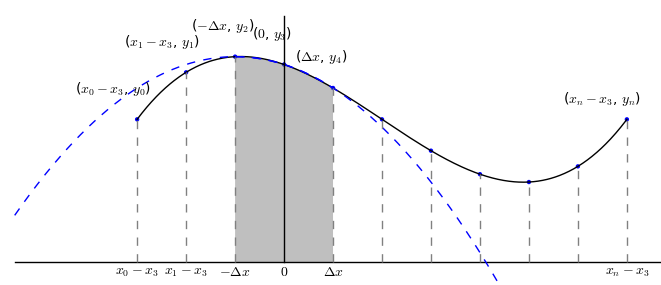
\includegraphics[scale=0.5]{shiftedSimpson}
\end{center}
So we see that instead of trying to fit a parabola to the points
\[(x_{2}, y_{2}), (x_3, y_3), (x_{4}, y_{4})\]
we can fit a parabola, \(q(x)\), to the points
\[(-\Delta x, y_{i-1}), (0, y_i), (\Delta x, y_{i+1})\]
so that the shifted parabola
\[p(x) = q(x - x_3)\]
satisfies
\begin{eqnarray*}
  p(x_2) &=& q(x_2 - x_3) = q(x_2 - (x_2 + \Delta x)) = q(-\Delta x) = y_2\\
  p(x_3) &=& q(x_3 - x_3) = q(0) = y_3\\
  p(x_4) &=& q(x_4 - x_3) = q(x_3 + \Delta x - x_3) = q(\Delta x) = y_4
\end{eqnarray*}
and
\[\int_{x_2}^{x_4} p(x)\dif x = \int_{-\Delta x}^{\Delta x} q(x)\dif x.\]
This small observation will simplify our task greatly.

Next, we set about computing all the areas we need.
The first thing we need is a parabola for each of \(i = 1, 3, 5, \ldots, n-1\).
For such an \(i\) we take the three points \((-\Delta x, y_{i-1})\), \((0,y_i)\), and \((\Delta x, y_{i+1})\).
The parabola we want will have the form
\[q(x) = Ax^2 + Bx + C\]
and it must satisfy the three equations
\begin{eqnarray*}
  y_i &=& q(0) = A(0)^2 + B(0) + C = C\\
  y_{i - 1} &=& q(-\Delta x) = A(\Delta x)^2 - B(\Delta x) + C\\
  y_{i + 1} &=& q(-\Delta x) = A(\Delta x)^2 - B(\Delta x) + C\\
\end{eqnarray*}
The first equation gives us \(C = y_i\).
If we add together the other two equations we see that
\[y_{i-1} + y_{i + 1} = 2A(\Delta x)^2 + 2y_i\]
so we have
\[2A(\Delta x)^2 = y_{i - 1} + y_{i + 1} - 2y_i.\]
This is enough information to solve for \(A\) and \(B\) in terms of \(y_{i - 1}\), \(y_i\), \(y_{i+1}\), and \(\Delta x\), but we can be a little more clever here.

Since \(x^2\) and the constant function are even functions, and \(x\) is an odd function, the area under \(q(x)\) on \([-\Delta x, \Delta x]\) is given by
\begin{eqnarray*}
  \int_{-\Delta x}^{\Delta x} q(x) \dif x &=& \int_{-\Delta x}^{\Delta x}(Ax^2 + Bx + C)\dif x\\
  &=& A\int_{-\Delta x}^{\Delta x} x^2 \dif x + B \int_{-\Delta x}^{\Delta x} x \dif x + C \int_{-\Delta x}^{\Delta x} \dif x\\
  &=& 2A \int_0^{\Delta x} x^2 \dif x + 0 + 2C \int_0^{\Delta x} \dif x\\
  &=& \frac{2}{3}A(\Delta x)^3 + 2C\Delta x\\
  &=& \frac{\Delta x}{3}\left(2A(\Delta x)^2 + 6C\right)\\
  &=& \frac{\Delta x}{3}\left(y_{i-1} + y_{i + 1} - 2y_i + 6y_i\right)\\
  &=& \frac{\Delta x}{3}\left(y_{i - 1} + 4y_i + y_{i + 1}\right).
\end{eqnarray*}
Now, as we observed above, the parabola
\[p(x) = q(x - x_i)\]
satisfies
\begin{eqnarray*}
  p(x_{i-1}) &=& q(x_{i - 1} - (x_{i-1} + \Delta x)) = q(-\Delta x) = y_{i-1}\\
  p(x_{i}) &=& q(x_{i} - x_{i}) = q(0) = y_{i}\\
  p(x_{i+1}) &=& q(x_i + \Delta x - x_i) = q(\Delta x) = y_{i+1}\\
\end{eqnarray*}
and
\[\int_{x_{i-1}}^{x_{i+1}} p(x)\dif x =
\int_{-\Delta x}^{\Delta x} q(x)\dif x =
\frac{\Delta x}{3}(y_{i - 1} + 4y_i + y_{i + 1})\]
Hence we have the approximation
\begin{eqnarray*}
  \int_a^b f(x)\dif x &\approx& \frac{\Delta x}{3}(y_0 + 4y_1 + y_2) +
  \frac{\Delta x}{3}(y_2 + 4y_3 + y_4) + \ldots \\
  &+& \frac{\Delta x}{3}(y_{n - 4} + 4y_{n - 3} + y_{n - 2}) + 
  \frac{\Delta x}{3}(y_{n-2} + 4y_{n-1} + y_n)\\
\end{eqnarray*}
We observe that the terms \(y_0\) and \(y_n\) will only appear once, and the terms \(y_1, y_3, \ldots, y_{n - 3}, y_{n-1}\) with odd subscript all appear with coefficient 4 exactly once.
All other terms with even subscript, \(y_{2j}\) for \(j = 1, 2, \ldots, n/2\), all appear twice: once in the approximation over the interval \([x_{2j-2}, x_{2j}]\) and once in the approximation over the interval \([x_{2j}, x_{2j + 2}]\).
Therefore we have
\begin{theorem}[Simpson's Rule]
  The integral
  \[\int_a^b f(x)\dif x\]
  can be approximated using \(n/2\) parabolas by
  \[S = \frac{\Delta x}{3}\left(y_0 + 4y_1 + 2y_2 + 4y_3 + \ldots + 2y_{n - 2}+ 4y_{n-1} + y_n\right),\]
  where
  \[\Delta x = \frac{b - a}{n},\]
  the interval \([a,b]\) is partitioned by
  \[x_0 = a,\, x_1 = a + \Delta x,\, x_2 = a + 2\Delta x,\, \ldots,\, x_{n-1} = a + (n-1)\Delta x,\, x_n = b,\]
  and \(y_i = f(x_i)\).
\end{theorem}

\begin{example}
  Use Simpson's rule to estimate
  \[\int_0^2 5x^4 \dif x\]
  using two parabolas.
\end{example}

\begin{proof}[Solution]
  First we compute
  \[\Delta x = \frac{2 - 0}{4} = \frac{1}{2}\]
  and so we have a partition
  \[x_0 = 0, x_1 = \frac{1}{2}, x_2 = 1, x_3 = \frac{3}{2}, x_4 = 2.\]
  The \(y\)-coordinates of the points we need are
  \[y_0 = 0, y_1 = \frac{5}{16}, y_2 = 5, y_3 = \frac{405}{16}, y_4 = 80.\]
  Thus the estimate is given by
  \begin{eqnarray*}
    S &=& \frac{1}{6}(0 + \frac{5}{4} + 10 + \frac{405}{4} + 80)\\
    &=& \frac{1}{24}(5 + 40 + 405 + 320)\\
    &=& \frac{770}{24}\\
    &=& \frac{2\cdot 5\cdot7\cdot 11}{2^3\cdot 3}\\
    &=& \frac{385}{12}\\
    &=& 32 + \frac{1}{12}.
  \end{eqnarray*}
\end{proof}

\subsection{Error Analysis}
Now that we have these two methods for approximation, the natural question to ask is, how good are these approximations?
\begin{theorem}
  If \(f^{\prime\prime}\) is continuous and \(M\) is any upper bound for the values of \(\abs{f^{\prime\prime}}\) on \([a,b]\), then the error, \(E_T\), in the trapezoidal approximation of
  \[\int_a^b f(x)\dif x\]
  for \(n\) trapezoids satisfies
  \[\abs{E_T} \leq \frac{M(b-a)^3}{12n^2}.\]

  If the fourth derivative, \(f^{(4)}\) is continuous and \(M\) is any upper bound for the values of \(\abs{f^{(4)}}\) on \([a,b]\), then the error, \(E_S\), in the Simpson's rule approximation of
  \[\int_a^b f(x)\dif x\]
  for \(n/2\) parabolas satisfies
  \[\abs{E_S} \leq \frac{M(b-a)^5}{180n^4}.\]
\end{theorem}
\begin{proof}
  Omitted.
\end{proof}

\begin{remark}
  Since both of these bounds rely on derivatives, it follows that any polynomial of degree at most 1, the Trapezoidal Approximation has no error, and for any polynomial of degree at most 3, the Simpson's Rule Approximation has no error, regardless of the choice of \(n\).

  For example, if we consider a polynomial
  \[\ell(x) = Mx + B\]
  then \(\ell^{\prime\prime}(x) = 0\), so for any interval \([a,b]\) we have
  \[\abs{E_T} \leq \frac{0(b-a)^3}{12n^2} = 0\]
  implies that \(E_T = 0\) and thus
  \[\int_a^b \ell(x)\dif x = T.\]

  Similarly, for any polynomial
  \[c(x) = Ax^3 + Bx^2 + Cx + D\]
  we have \(c^{(4)}(x) = 0\), so
  \[\abs{E_S} \leq \frac{0(b-a)^5}{180n^4} = 0\]
  implies that \(E_S = 0\) and thus
  \[\int_a^b c(x)\dif x = S.\]
\end{remark}

\begin{example}
  As an interesting special case of the last statement in the remark, consider the following cubic polynomial.
  Let \(a < c < b\) be real numbers and define
  \[p(x) = (x -a)(x-b)(x - c) = x^3 - (a + b + c)x^2 +  (ab + ac + bc)x  - abc.\]
  Take \(n = 2\), so then we have
  \begin{eqnarray*}
    \int_a^b p(x)\dif x &=& (p(a) + 4p\left(a + \frac{b-a}{2} + p(b)\right)\frac{b-a}{6}\\
    &=& 4p\left(\frac{a + b}{2}\right)\frac{b - a}{6}
  \end{eqnarray*}
  In particular, if \(c = \frac{a + b}{2}\), then we see that
  \[\int_a^b p(x)\dif x = 0.\]

  Concretely, we could take the polynomial
  \[p(x) = (x + 2)(x - 2)(x - 6) = x^3 - 6x^2 - 4x + 24\]
  and
  \[\int_{-2}^6 p(x)\dif x = 0\]
  which tells us that there is a certain symmetry about a degree three polynomial with evenly spaced roots!
  That is to say, in the graph
  \begin{center}
    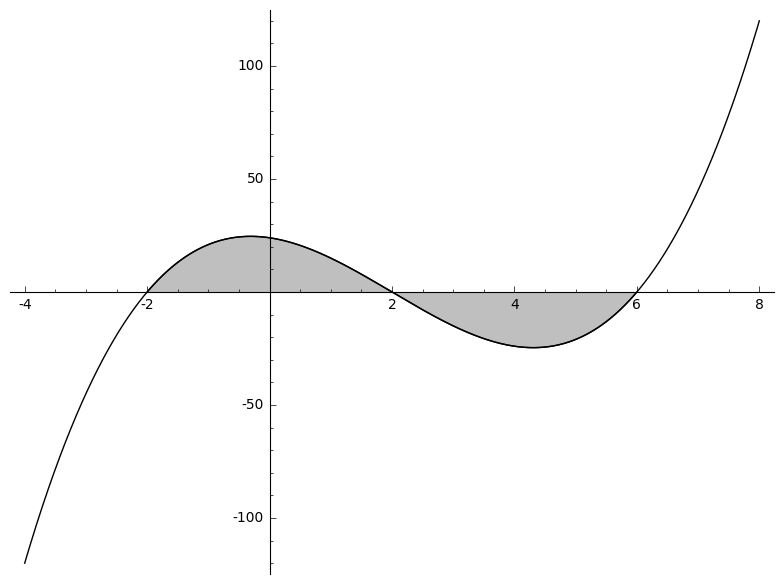
\includegraphics[scale=0.5]{cubic}
  \end{center}
  the two shaded regions are the same size.
\end{example}

\begin{example}
  Find an upper bound for the error in estimating
  \[\int_0^2 5x^4\dif x\]
  using Simpson's Rule with \(n = 4\).
\end{example}

\begin{proof}[Solution]
  Since we're using \(f(x) = 5x^4\), we note that
  \[f^{(4)}(x) = 210 = M\]
  serves as an upper bound on \([0,2]\), so
  \[\abs{E_S} \leq \frac{120(2)^5}{180(4)^4} = \frac{120}{180 \cdot 2^3} = \frac{2}{3\cdot8} = \frac{1}{12}\]
\end{proof}

\begin{example}
  Determine the number of subintervals, \(n\), needed to estimate
  \[\int_0^2 5x^4\dif x\]
  to an error of magnitude less than \(10^{-4}\) using Simpson's Rule.
\end{example}

\begin{proof}[Solution]
  We want to have
  \[\abs{E_S} \leq \frac{M(b-a)^5}{180n^4} = \frac{120(2^5)}{180n^4} = \frac{2^6}{3n^4}< 10^{-4}.\]
  So, all we need to do is require that
  \[\frac{2^6\cdot 10^4}{3} < n^4\]
  or, equivalently, that
  \[\frac{\sqrt[4]{2^6}\sqrt[4]{10^4}}{\sqrt[4]{3}} = \frac{2^{3/2}\cdot 10}{\sqrt{4}{3}} < n.\]
  Since
  \[\frac{2^{3/2}\cdot 10}{\sqrt{4}{3}} \approx 21.5\]
  it follows that we can ensure the error is less than \(10^{-4}\) by taking \(22 \leq n\).
\end{proof}
\end{document}
